\subsection{Tourism Domain and Lodging Economics}

\paragraph{Tourism and its components.}
Tourism is one of the largest industries in the world, yet it is also, in the words of Goeldner and Ritchie, ``\emph{a complex phenomenon, one that is extremely difficult to describe succinctly}'' (p.~14)~\cite{goeldner2009}. The textbook organises the phenomenon into four interrelated components --- the tourist, the natural resources and environment, the built environment, and the operating sectors of the tourism industry --- as shown in Figure~\ref{fig:tourism-phenomenon} (Fig.~1.2, p.~14).

The heart of the model is the tourist: ``\emph{the very heart of the tourism phenomenon model is unequivocally the tourist and the travel experiences that he or she seeks}'' (p.~15). For revenue management this has a direct meaning: each tourist is a decision maker who chooses whether to book a room, at what price, at what time, and through which channel. Around the tourist, the natural resources and environment of a destination --- physiography, climate, culture --- are largely immutable: they cannot be adjusted to raise visitor arrivals (p.~14)~\cite{goeldner2009}, and this immutability is the root of \emph{seasonality}. The built environment distinguishes \emph{infrastructure} --- roads, sewage systems, communication networks built to meet the needs of local residents --- from the \emph{tourism superstructure}: ``\emph{facilities that have been developed especially to respond to the demands of visitors}'' (p.~17), with hotels listed as the first example. Crucially, ``\emph{the characteristics of components of the superstructure are essentially determined by visitor wishes rather than resident desires}'' (p.~17): a hotel's pricing, room types, and services must reflect what visitors want and are willing to pay for. Finally, the operating sectors --- transportation, accommodation, food services, attractions, events, and others --- are ``\emph{what many of the general public perceive as `tourism'}'' (p.~19)~\cite{goeldner2009}; Figure~\ref{fig:operating-sectors} shows the textbook's view of these sectors. Among them, ``\emph{tourists need a place to stay and be fed, so the accommodation sector and the food service sector are important supply components}'' (p.~383)~\cite{goeldner2009}, and our problem belongs to the accommodation sector, which Chapter~6 of the textbook develops.

\begin{figure}[H]
\centering
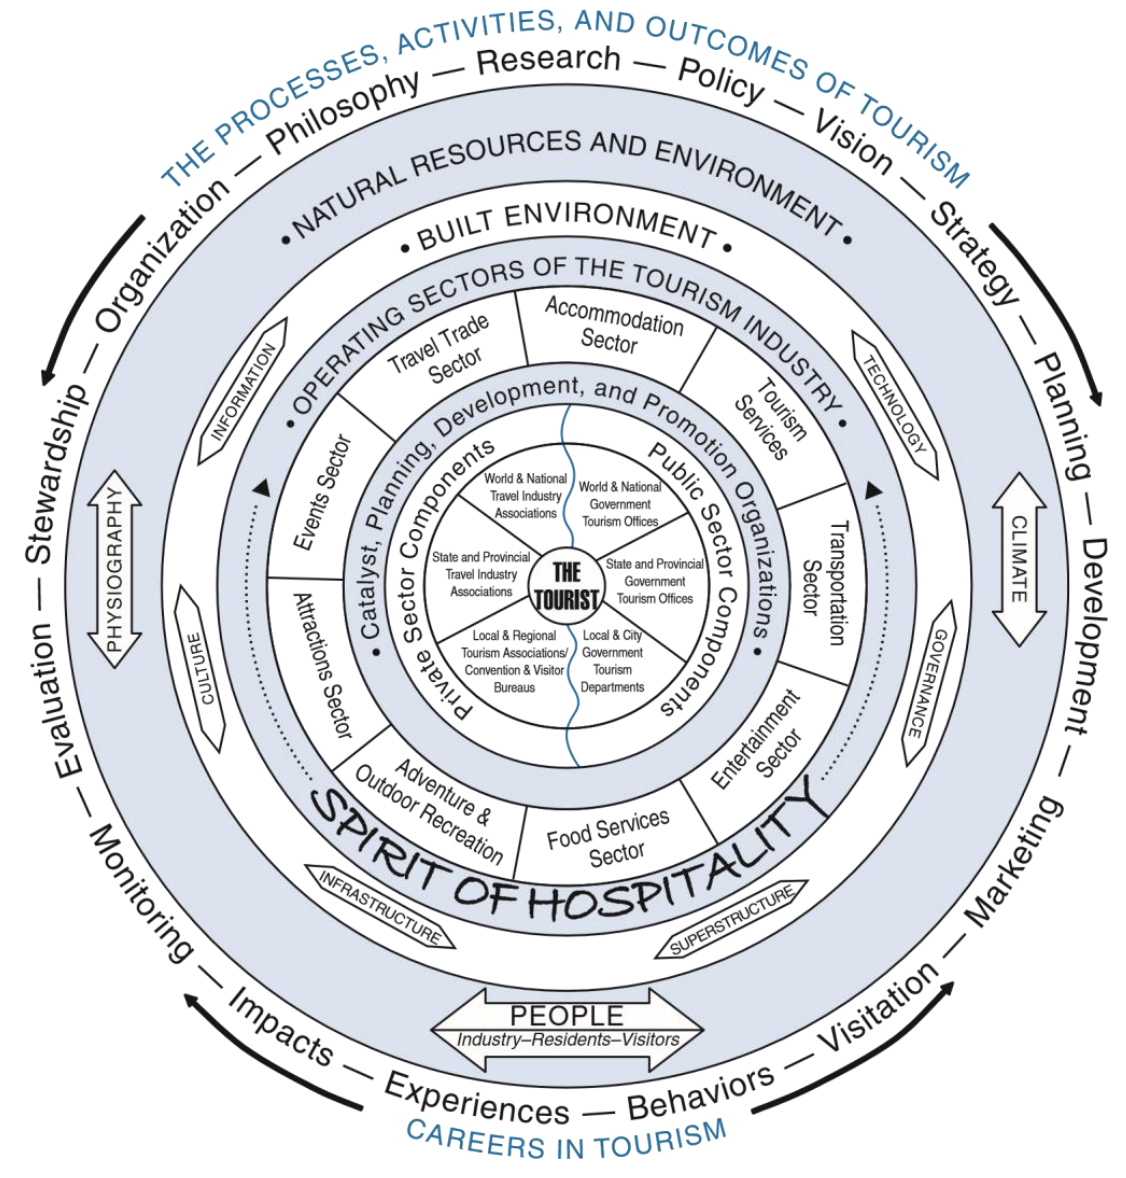
\includegraphics[width=0.52\textwidth]{figures/1-introduction/tourism-phenomenon.png}
\caption{The tourism phenomenon: components of tourism and tourism management (Goeldner \& Ritchie, Fig.~1.2, p.~14)~\cite{goeldner2009}.}
\label{fig:tourism-phenomenon}
\end{figure}

\begin{figure}[H]
\centering
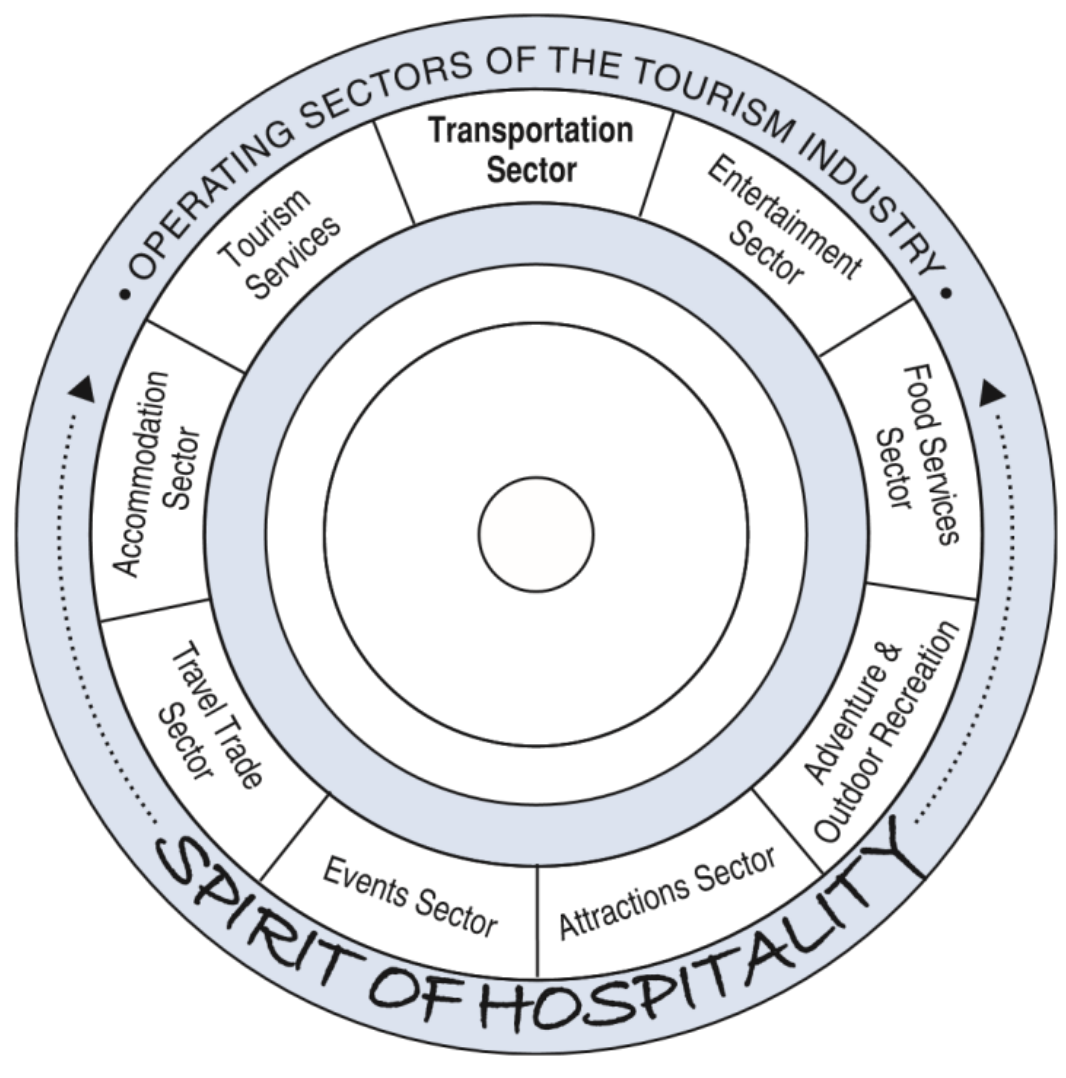
\includegraphics[width=0.5\textwidth]{figures/1-introduction/operating-sectors.png}
\caption{Operating sectors of the tourism industry --- accommodation is one of them (Goeldner \& Ritchie, Ch.~1)~\cite{goeldner2009}.}
\label{fig:operating-sectors}
\end{figure}

\paragraph{The lodging industry.}
Providing overnight accommodation ``\emph{goes back into antiquity; it is the world's oldest commercial business}'' (p.~180). The sector spans a wide range of accommodation structures --- hotels, motels, suites, resort properties, bed-and-breakfasts, timeshare, and camping (Figure~\ref{fig:accommodation-structures}; Ch.~6)~\cite{goeldner2009} --- of which our project addresses the hotel segment. The scale of the U.S.\ sector alone, per the AH\&LA 2007 Lodging Industry Profile cited in the textbook, is ``\emph{47{,}135 properties, 4.4 million rooms, \$133.4 billion in sales, \$26.6 billion in pretax profit, 63.3 percent average occupancy rate, and \$61.93 revenue per available room}'' (p.~156). An average occupancy of 63.3\% means that more than one-third of all hotel rooms go unsold every night --- a substantial, recurring revenue gap.

\begin{figure}[H]
\centering
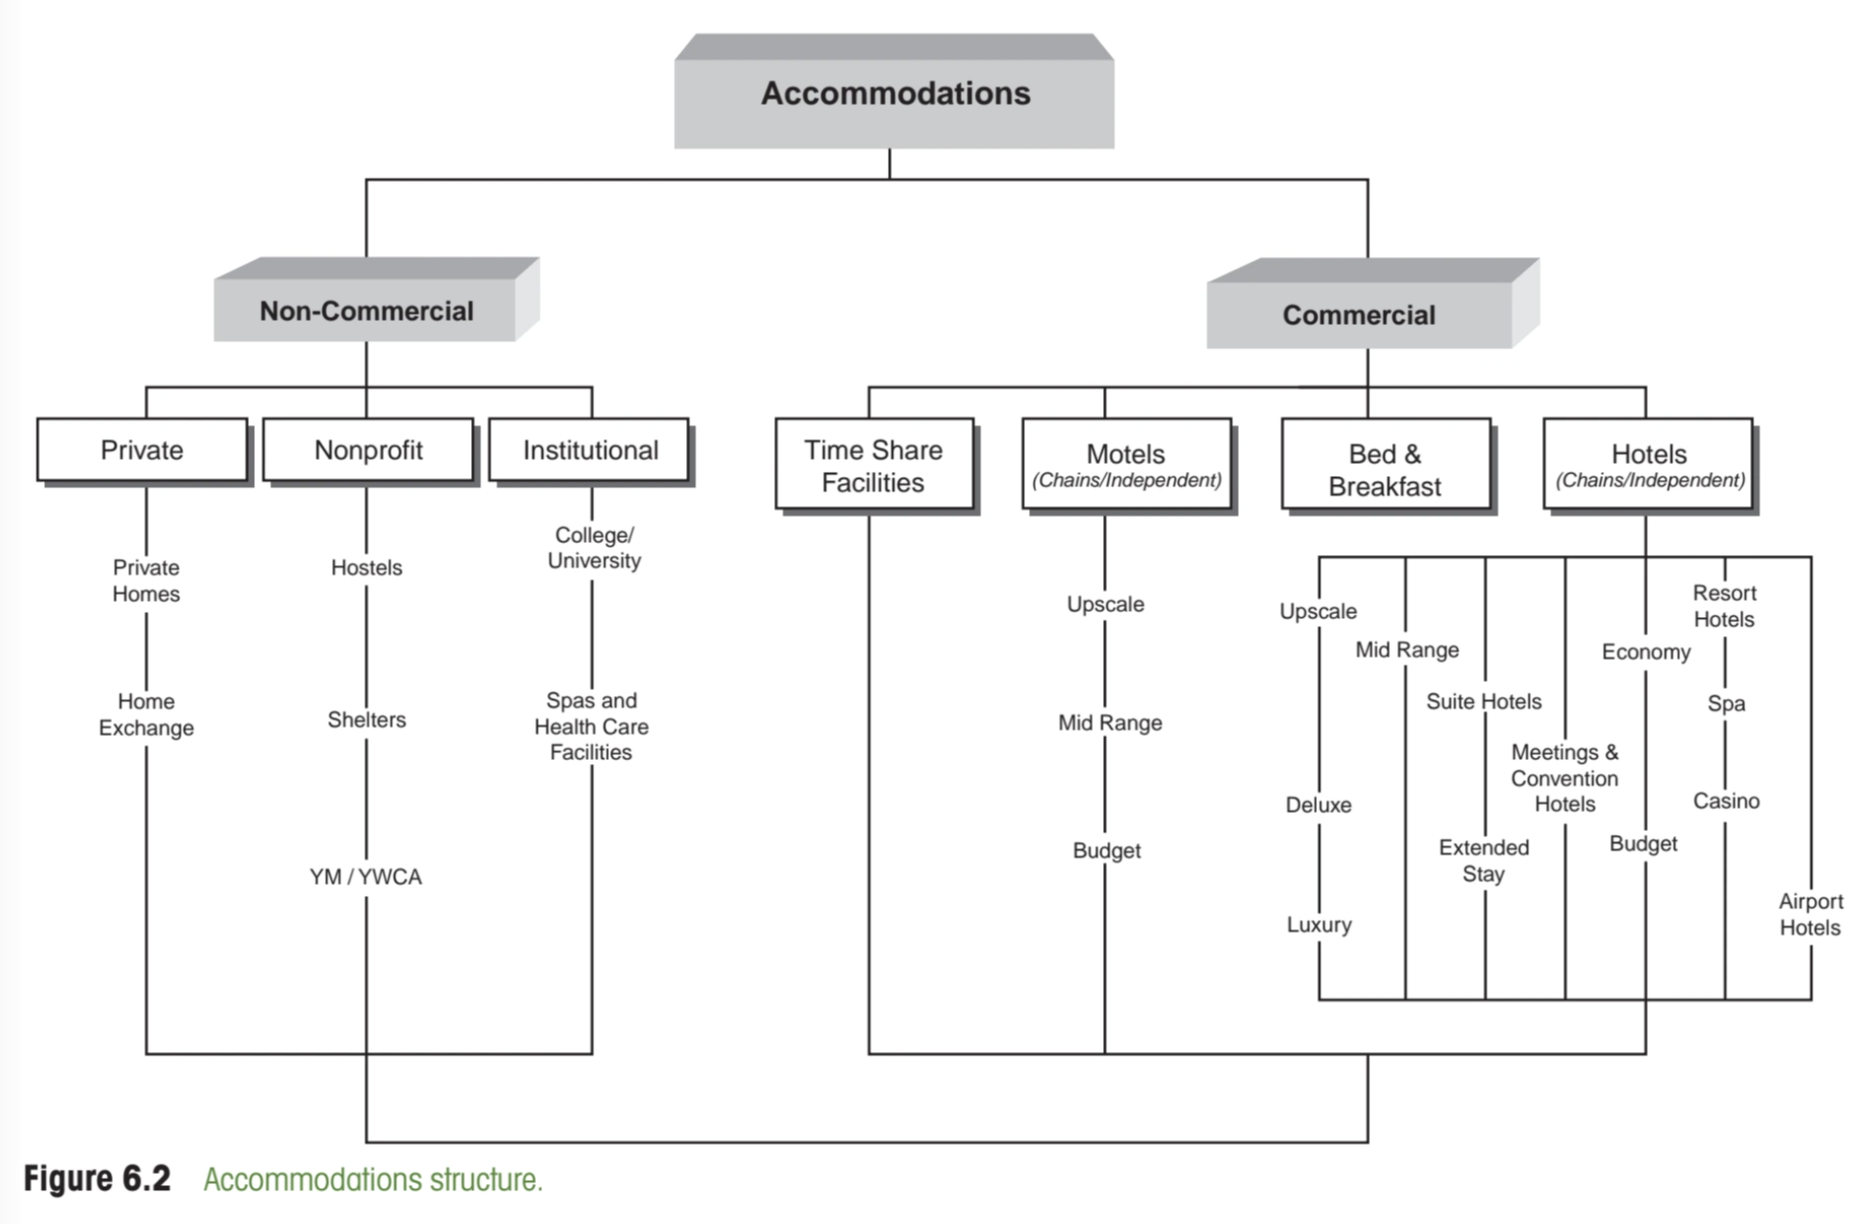
\includegraphics[width=0.7\textwidth]{figures/1-introduction/accommodation-structures.png}
\caption{Structures of the accommodation sector (Goeldner \& Ritchie, Ch.~6)~\cite{goeldner2009}.}
\label{fig:accommodation-structures}
\end{figure}

\paragraph{Key performance indicators.}
The textbook's glossary defines the three metrics that every revenue manager monitors (p.~186): \textbf{ADR} (Average Daily Rate) is ``\emph{guestroom revenue for a given period divided by total number of occupied rooms}''; \textbf{Occupancy} is ``\emph{available rooms occupied for a given period. Computed by dividing the number of rooms occupied by the number of rooms available}''; and \textbf{RevPAR} (Revenue Per Available Room) is ``\emph{guestroom revenue for a given period divided by total number of available rooms. A simple way to calculate is to multiply the occupancy times the room rate}''. These three metrics are tightly coupled: raising rates (higher ADR) may reduce occupancy, while lowering rates to fill rooms may reduce ADR. RevPAR is the composite measure that captures this trade-off, and it is the optimisation target of the system developed in this project.

\paragraph{Customer segments.}
``\emph{Who is the typical lodging customer? According to the AH\&LA, 44 percent are business travelers and 56 percent are leisure travelers}'' (p.~156). The typical business room-night is generated by a male (65\%) aged 35--54, earning \$85{,}900 per year, travelling alone (56\%), and paying \$112 per night; the typical leisure room-night involves two adults, earning \$77{,}100, travelling by automobile (77\%), and paying \$103 per night. The difference in price sensitivity and booking behaviour between these segments is the economic foundation for differentiated pricing: the same room is worth different amounts to different customers.

\paragraph{Structural characteristics of supply, cost, and demand.}
Revenue management is both necessary and difficult because six structural conditions hold simultaneously in hotel lodging, and each grounds one part of the solution developed in this project.

\emph{Product and capacity constraints.} First, the product is \textbf{perishable}: an unsold room-night cannot be stored or resold --- ``\emph{the utilization of perishable assets}''~\cite{mcgill1999}, ``\emph{the perishable nature of hotel rooms}''~\cite{amadeus2023} --- the property that drove the airline industry to originate yield management~\cite{rothstein1971} and that is shared by all capacity-constrained service businesses~\cite{kimes1989} (Table~\ref{tab:perishable}). Second, \textbf{capacity is relatively fixed}: a hotel cannot add or remove rooms on a daily basis; accommodations ``\emph{must be available in sufficient quantity to match the demand of the travelers who arrive at the destination}'' (p.~388)~\cite{goeldner2009}.

\emph{Economics and cost structure.} Third, the industry combines \textbf{high fixed costs with low variable costs}: ``\emph{the high fixed cost and low variable cost typically associated with the hotel industry means that a large portion of this revenue increase flows directly to the bottom line}''~\cite{anderson2012}. This is the economic motor of the problem: because the marginal cost of selling one more room is close to zero, every euro of revenue that pricing and allocation recover converts almost entirely into profit.

\emph{Market and booking dynamics.} Fourth, \textbf{demand fluctuates} predictably across seasons and days of the week while supply stays constant, creating excess demand in peaks and excess capacity off-peak --- an imbalance rooted, in the textbook's terms, in the immutability of a destination's natural resources (p.~14)~\cite{goeldner2009}. Fifth, demand is \textbf{segmentable}: ``\emph{RM is about a hotel's ability to segment its consumers and price and control room inventory differently across these segments --- in essence practicing some form of price discrimination}''~\cite{anderson2012}; the willingness-to-pay gap between the business and leisure segments documented above makes this concrete, and rate fences (time of purchase, refundability, affiliation) keep the segments separated~\cite{anderson2012}. Sixth, bookings occur \textbf{in advance of consumption}, across a booking window measured in days before arrival: ``\emph{RM systems use existing reservations on hand (ROH) to develop forecasts for future arrivals days}'', with booking and pace curves presented as functions of days before arrival~\cite{anderson2012}. The window is recorded in the data itself (booking lead time)~\cite{antonio2019} and is where the overbooking model of this project measures its show-up probabilities.

Together, the first four conditions explain why the problem exists --- a perishable, fixed-capacity product with near-zero marginal cost, facing uneven demand --- and the last two why it is tractable: segmentation provides the price lever, and the booking window provides the observation and intervention timeline.

\begin{table}[H]
\centering
\caption{Perishable inventory across capacity-constrained service industries~\cite{kimes1989}.}
\label{tab:perishable}
\begin{tabular}{@{}ll@{}}
\toprule
\textbf{Industry} & \textbf{Perishable inventory} \\
\midrule
Hotels & Room for a given night \\
Airlines & Seat on a given flight \\
Tours & Seat on a given departure \\
Restaurants & Table for a given service period \\
Events & Ticket for a given performance \\
\bottomrule
\end{tabular}
\end{table}

\paragraph{Measuring demand.}
Chapter~13 of the textbook frames demand measurement for tourism: ``\emph{demand for travel to a particular destination will be a function of the person's propensity to travel and the reciprocal of the resistance of the link between origin and destination areas. Thus, $D = f(\text{propensity}, \text{resistance})$}'' (p.~414). Among the possible measures, the textbook is explicit about the unit that matters for our sector: ``\emph{data on visitor-days and visitor-nights are much more valuable to tourism planners than are data on the number of arrivals}'' and ``\emph{hotel and other accommodations people want data on visitor-nights}'' (p.~418). This is the domain justification for the booking-night grain of the data warehouse designed in Section~3.2. Money spent is ``\emph{the most meaningful measure}'' but also ``\emph{the most difficult measure to obtain}'' (Ch.~13)~\cite{goeldner2009}.

\paragraph{The industry's response: yield management.}
Against this background, the textbook records the industry's response as a clear trend: ``\emph{Other trends are the increased use of central reservation systems, emphasis on service, and the use of yield management techniques}'' (p.~190). The glossary defines yield management as ``\emph{the use of pricing and inventory controls, based upon historical data, to maximize profits by offering varying fares over time for the same product}'' (p.~698), and the classic operations-management formulation states its objective plainly: ``\emph{the objective of yield management is to maximize the revenue or yield of the firm. A good yield management system will help the firm decide how much of each type of inventory (whether it be seats on an airplane, rooms in a hotel, or cars in a rental car fleet) to allocate to different types of demand}''~\cite{kimes1989}. The economics justify the effort: hotel revenue management ``\emph{has been shown to increase revenue by 2 to 5 percent}''~\cite{anderson2012}; commercial revenue management decision support systems report gains of approximately 6\%~\cite{boyd2003}, and American Airlines' pioneering system 4--7\%~\cite{smith1992}. In the language of operations research, revenue management is ``\emph{the utilization of perishable assets to maximize a firm's revenues over a short-term horizon given that costs are effectively fixed over that horizon}''~\cite{mcgill1999} --- confirming conditions 1 and 3 above (perishable inventory, and the high-fixed-cost/low-variable-cost structure) from the operations-research tradition. Contemporary industry guidance confirms that revenue management now rests on four foundational principles --- \emph{segmentation}, \emph{forecasting}, \emph{optimisation}, and \emph{distribution}~\cite{amadeus2023} --- which map directly onto the models developed in this project.
